% This file is the Latex source of the Big Data course project
% report. The project contributors are Ali Alavi, Rolf jagerman
% and Ken Tsay.
% The report is written by Ali Alavi, Rolf Jagerman.

%
\documentclass{llncs}
%

\usepackage{graphicx} % for importing images
\usepackage{caption}
\usepackage{subcaption} % for subfigures
\captionsetup{compatibility=false} % to make subfigures compatible with template

\usepackage{url} % for URL references
\usepackage{float} % helps with locating the 
\usepackage[T1]{fontenc}  % providing font encoding
% used for drawing the diagrams
%
\begin{document}
%
\mainmatter              % start of the contributions
\pretolerance=10000  % This avoids long lines
\pagestyle{headings}
%\hyphenation{}

%
\title{Automatic News Generation Based on Twitter}
%
\titlerunning{Automatic News Generation Based on Twitter}  % abbreviated title (for running head)
%                                     also used for the TOC unless
%                                     \toctitle is used
%
\author{Ali Alavi\inst{1} \and Rolf Jagerman\inst{1} \and
Tsay Kai-En\inst{1}}
%
\authorrunning{Ali Alavi, Rolf Jagerman and Tsay Kai-En} % abbreviated author list (for running head)
%
%
\institute{ETH Z\"urich, Z\"urich, Switzerland\\
\email{alavis@ethz.ch, \{rolfj, tsayk\}@student.ethz.ch}
}

\maketitle              % typeset the title of the contribution
%

\section{Introduction}
% todo
This report presents the current status of the project \textbf{Automatic News Generation Based on Twitter}, for \textbf{Big Data} course (code \textit{263-3010-00L}). This project tries to answer the following questions: 
\textit{Can we automatically generate news headlines based on public twitter posts? Can this method of news generation perform better than the available news agencies, in terms of speed, reliability and so on?}

We tackle this problem by taking the following steps:

\begin{enumerate}
	\item \textit{Data collection: }Gathering a large set of twitter posts and news headlines 
	\item \textit{Building a classifier: }Use the news headlines to train a classifier
	\item \textit{Labeling the tweets: }Label each tweet using the classifier we previously trained
\end{enumerate}

A big picture of the system is depicted in Figure ~\ref{fig:A big picture of the system}. In the rest of this report we will elaborate how we implement the solution in a scalalaby way on Spark. 

\begin{figure}[H]
	\centering
	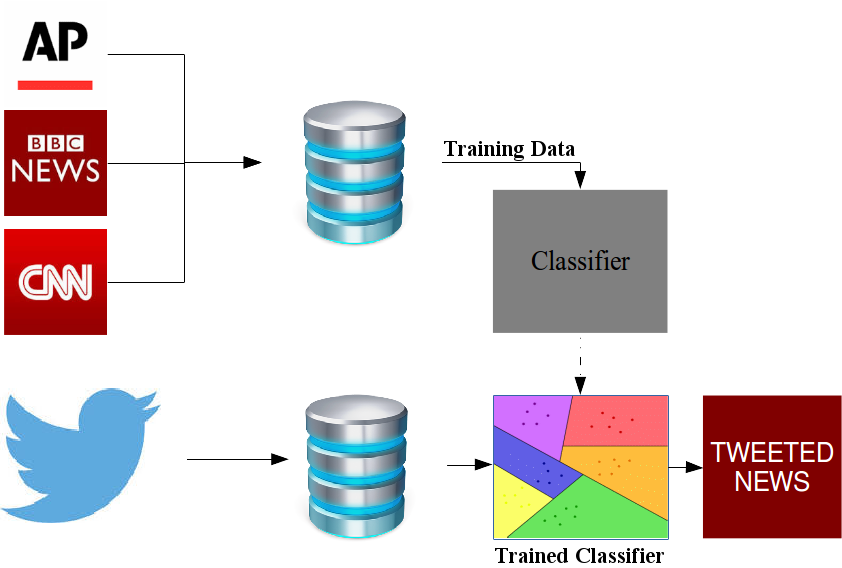
\includegraphics[width=0.8\textwidth]{images/bigpicture.png} 
	\caption{A big picture of the system}
	\label{fig:A big picture of the system}
\end{figure}



\section{Data model}
% todo
...


\section{Design of the system}
System architecture is depicted in Figure ~\ref{fig:Architecture design of the system}. The data storage component is on Amazon S3, and the data process platfrom is on Apache Spark. 

\begin{figure}[H]
	\centering
	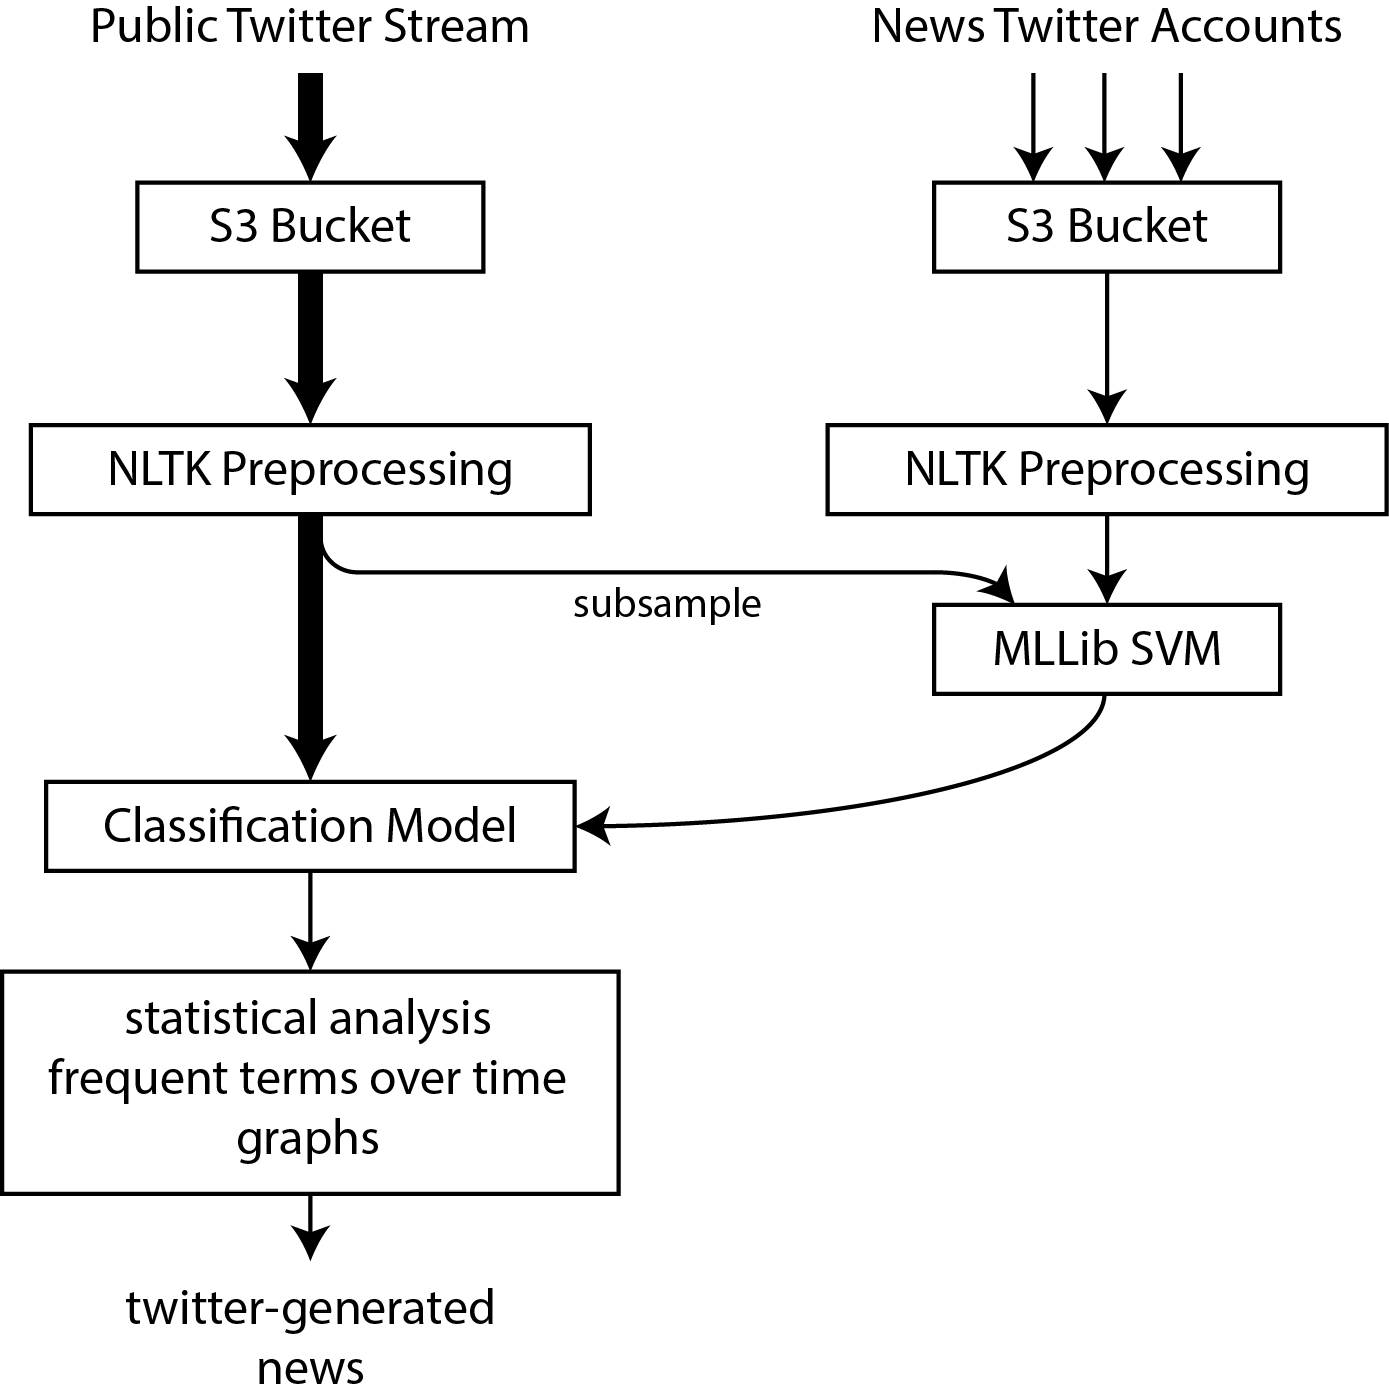
\includegraphics[width=0.8\textwidth]{images/system_arch.png} 
	\caption{Architecture design of the system}
	\label{fig:Architecture design of the system}
\end{figure}

\subsection{Data storage}
We stored around 600G of the twitter stream data on Amazon S3. Differ from previous work, we integrate the data collecting script with s3cmd tool, which is a command line tool and client for uploading, retrieving and managing data in Amazon S3~\cite{s3cmd}, and direct uploaded the twitter streamming data into S3 bucket. This benefit the whole system cause we can load the large training and prediction dataset via using S3 protocol into our Spark instance. 

\subsection{Data process platform}
Our data processing consists of two separate phases. At first, we classify the tweets by running it on Spark, on top of Amazon Elastic Mapreduce(EMR). In the begining we were running Spark on Aamzon EC2, we create ...
 
\subsection{Platform}

\section{Results}

\subsection{Classification performance}

In our previous report, we measured our news classifier's performance by using precision, recall and f1-score. These scores are shown in table \ref{tbl:oldclassifier}.

\begin{table}
	\begin{center}
		\begin{tabular}{|r|r|r|r|r|} \hline
			class  & precision   & recall & f1-score  & support \\ \hline
			technology    &   1.00 &     0.08  &    0.14   &   6195 \\
			sports   &    1.00   &   0.03   &   0.07   &   6365 \\
			politics   &    1.00  &    0.10   &   0.18   &   6376 \\
			avg / total  &     1.00   &   0.07  &    0.13   &  18936 \\ \hline
		\end{tabular}
	\end{center}
	\caption{Old classification performance over the three trained categories}
	\label{tbl:oldclassifier}
\end{table}

It was evident that the classifier was not performing optimally. The high precision measures were offset by the extremely low recall measures. This meant that the classifier was only predicting the relevant labels for a few tweets and discarding most of them. This was likely the result of training on an imbalanced data set.

The new classifier was trained on roughly two to three times as much data. Additionally, we ensured that each classifier in the one-vs-all approach was trained on roughly equally many positive and negative datasamples. The scores for the classifier are shown in table \ref{tbl:newclassifier}

\begin{table}
	\begin{center}
		\begin{tabular}{|r|r|r|r|r|} \hline
			class  & precision   & recall & f1-score  & support \\ \hline
			technology    &   0.78 &     0.92  &    0.84   &  25343 \\
			sports   &    0.75   &   0.73   &   0.74   &   25343 \\
			politics   &    0.83  &    0.75   &   0.79   &   25343 \\
			avg / total  &     0.79   &   0.80  &    0.79   &  76029 \\ \hline
		\end{tabular}
	\end{center}
	\caption{New classification performance over the three trained categories}
	\label{tbl:newclassifier}
\end{table}

Although the precision of the classifier has gone down, our recall has increased a lot. This means that, although some predictions are wrong, we have a lot more predictions to work with.

Despite scaling up the entire system, the amount of available training data did not increase significantly. The changes in performance are not due to an increase of data, but are more likely attributed to training on a more balanced data set.

\subsection {Post-processing the classified results}
% time series
Although the classifier manages to classify the tweets in the mentioned categories, these classified outputs are not essentially news headlines. This is due to the fact that the classifier classifies the tweets individually, while an important property of news-related tweets is their frequency of appearance in a given timeframe. Hence, we need to perform some temporal analysis of the classified tweets.

We perform analysis by sampling the tweets, with a rate of \textit{R}, then tokenizig the classified tweets and filtering out the less frequent nouns. In this way, we manage to filter out lots of noisy outputs of the classifier. Afterwards, we look into different slope of the time series, and identify top surging topics as news-worthy topics, which can be presented to the users.

Selecting the sampling rate R is non-trivial, as it depends on the life time of each news, which varies based on the news topic, scale (global or regional), and so on. Despite that, we managed to see reasonable results with sampling frequencies of 1 hour. See Figure \ref{fig:Political news topic prediction using time series analysis, with a sampling frequency of 1 hour}.





\begin{figure}[H]
	\centering
	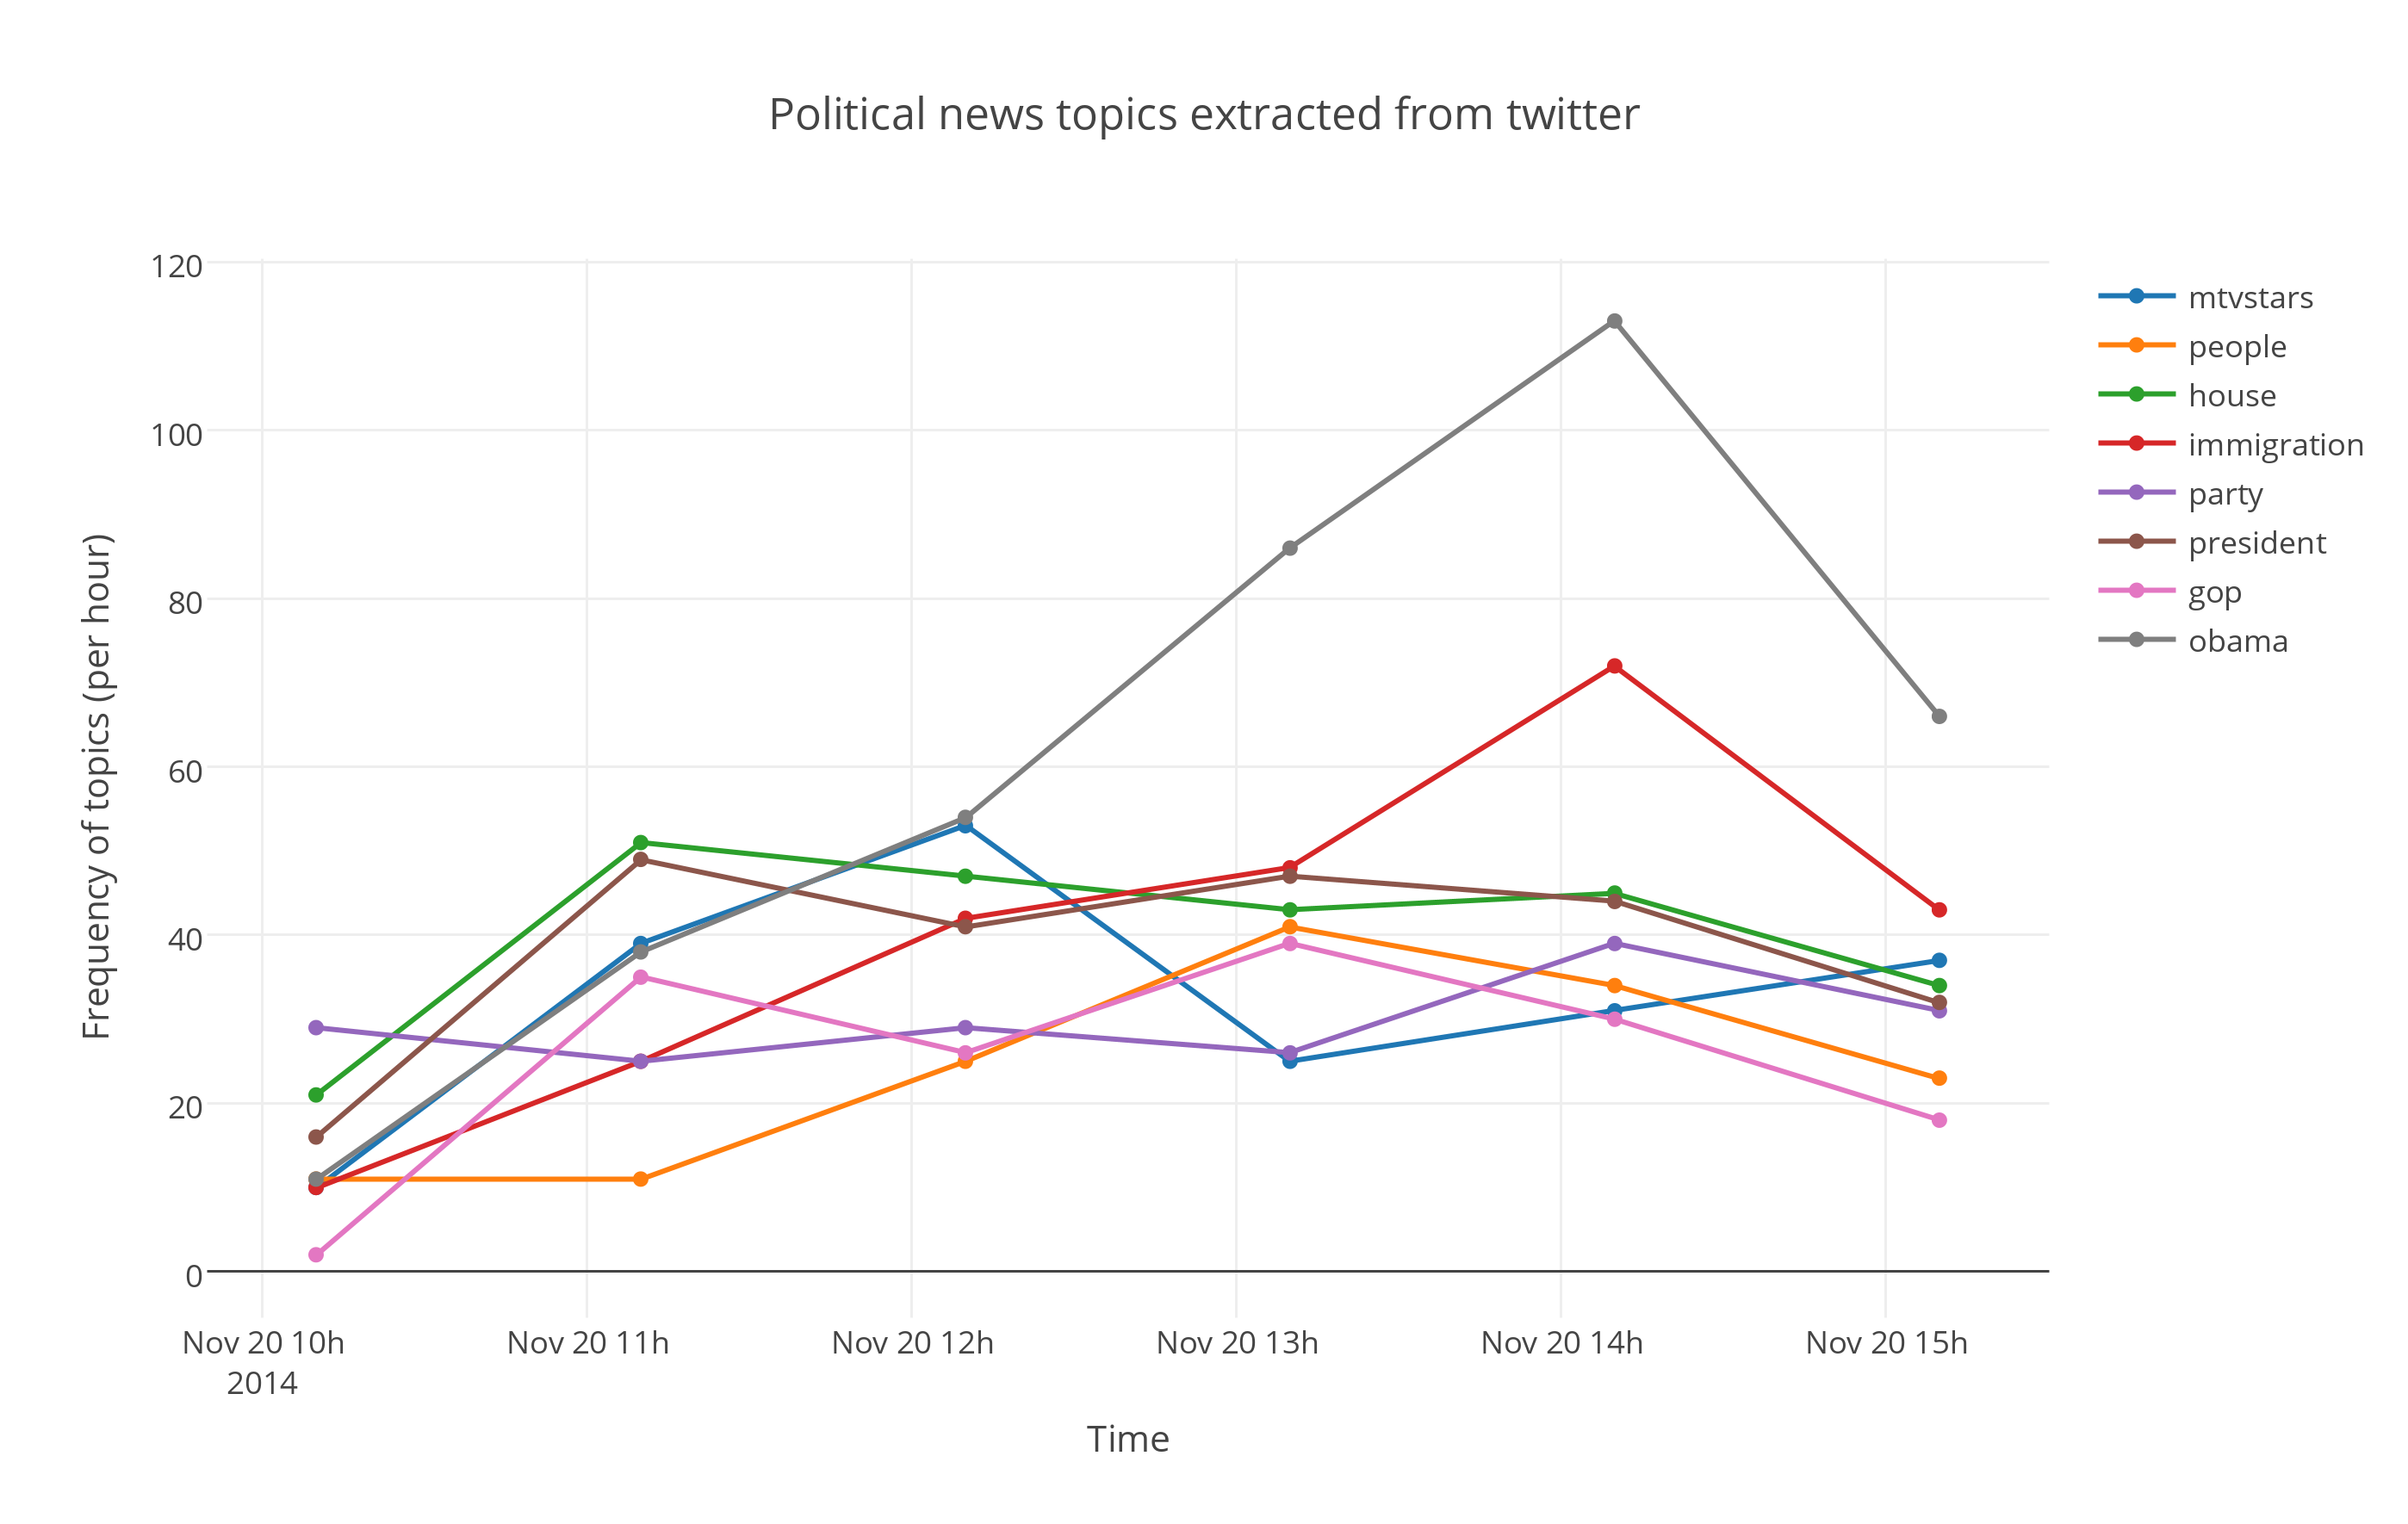
\includegraphics[width=0.8\textwidth]{images/political_news_topics_extracted_from_twitter.png} 
	\caption{Political news topic prediction using time series analysis, with a sampling frequency of 1 hour}
	\label{fig:Political news topic prediction using time series analysis, with a sampling frequency of 1 hour}
\end{figure}

\subsection{Prediction scalability}

Our main goal in this part of the project was to scale up our prediction capability. We want to use our trained classifier to quickly classify all of the collected tweets. We were able to classify 600GB of tweets in roughly 10 hours using 20 Amazon EC2 m1.medium instances. The Spark Map-Reduce framework created 10,702 tasks. Each of these tasks independently computes the predictions on a part of the dataset and write the results to a file on s3. A single task takes on average $65.4 (\pm 20.6)$ seconds to complete. Since we were restricted to 20 EC2 instances, this takes about 10 hours in total. With sufficiently available instances, this computation could have been done in minutes instead of hours.

\section{Future Work}


\bibliographystyle{plain}
\bibliography{report.bib}

\end{document}